\section{Scrum is not just about standing up and burning down}
This section highlights the most important principles of the Agile
Manifesto.

{\bf Individuals and interactions} \emph{over processes and tools.} Developing
software is an intellectual and creative process, which is challenging and spectacularly
complicated. Managers do not make any differentiation between a software
developer and a house builder. They assume they can plug and play people into a
software project as they can in the house building industry, which is obviously
not the same thing. Agile teams are most commonly compared to
sports teams, which can only win if the team members play together. Teamwork
requires by definition a great deal of communication skills. Processes are
important, but not vital. If you had a choice between an NBA level basketball
team and a group of very smart, athletic and toll people who never heard of
basketball before, but got it explained in detail just prior to the match, on
which team would you bet your money on? And always remember, that although tools
are helpful a fool with a tool is still a fool.

{\bf Working software} \emph{over comprehensive documentation.} The goal of
software development is software, not documentation, otherwise it would be called
documentation development.\cite{Ambler200204} Documentation is important, but
not a priority. And why should it be? If you think about it, working software is
even more explanatory than a technical, gibberish document.

{\bf Customer collaboration} \emph{over contract negotiation.} Developing software is a
creative process and the fact that software developers are the only stakeholders
in the software project is nothing more than an illusion. The customer {\bf
develops} ideas and the software developer implements them. Thus the customer
becomes a vital part of the team and communication skills are required yet
again. The customer has to be creative himself. Since creativity is an iterative
process, there is just no way, the customer could communicate his wishes to the
software developer upfront. And even if he could, would the software developer
go ahead and build the whole system in one sit?

{\bf Responding to change} \emph{over following a plan.} The fact that change {\bf is}
the state in the software world is undeniable. Technology, business environment,
skills, domain understanding change over time and there is nothing you can do
about it. In fact you should embrace change and act now instead of planning for
tomorrow to paraphrase the surprisingly effective way of thinking:
\enquote{Implement for today, design for tomorrow.}\cite{BeckAndres200411}

\section{Extreme Programming}
This section introduces XP and explains the origins of the \emph{extreme}
part in its naming.

The main purpose of XP is to reduce project risk, making everyone happy on its
way. The programmers work on tasks that really matter. These tasks are fun and
fun is the reason why they got into programming in the first place. In
addition to that, they never have to make important decisions on their own and
therefore become fearless of change. The customers and managers receive rapid
feedback, which gives them the ability to steer the project in the right
direction or even entirely change the course of action.\cite{BeckAndres200411}

XP maximizes agile principles and practices buy boosting them to extreme levels
and this is where the name comes from:
\begin{itemize}
\item If code reviews are good, we'll review code all the time (pair
programming).
\item If testing is good, everybody will test all the time (unit testing), even
the customers (functional testing).
\item If design is good, we'll make it part of everybody's daily business
(refactoring).
\item If simplicity is good, we'll always leave the system with the simplest
design that supports its current functionality (the simplest thing that could
possibly work).
\item If architecture is important, everybody will work defining and refining
the architecture all the time (metaphor).
\item If integration testing is important, then we'll integrate and test
several times a day (continuous integration).
\item If short iterations are good, we'll make the iterations really, really
short - seconds and minutes and hours, not weeks and months and years (the
Planning Game).\cite{BeckAndres200411}
\end{itemize}

\section{Agile Modeling}
This section introduces AM and explains its goals, but before jumping into AM we
discuss why bother with modeling at all.

Models are artifacts, which help you understand whay you are building or aid the
communication with your team. And since communication is so important to an
agile team (or any team for that matter), modeling is also important.

\subsection{What is AM?}
AM is not a complete software process like XP. Instead AM is a modification for
a software process as presented in the following figure.
 \begin{figure}[h]
  \caption[AM Scope]{AM Scope\cite{AM}}
  \label{jee}
  \center
  	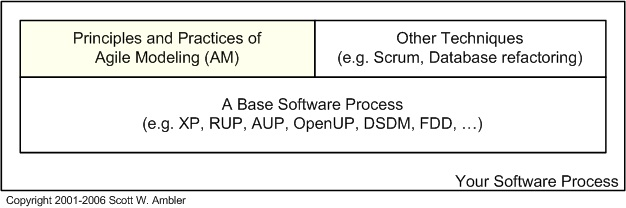
\includegraphics[scale=0.5]{../resources/amScope.jpg}
\end{figure}
AM is all about modeling and documentation. AM does not show how to create new
models, but how to apply existing modeling techniques. AM
\begin{itemize}
\item is an attitude, not a prescriptive process
\item is a supplement to existing methods; not a complete methodology
\item is complementary to other modeling processes
\item is a way to work together effectively to meet the needs of project
stakeholders
\item is effective and is about being effective
\item is something that works in practice; isn't an academic theory
\item is not a silver bullet
\item is for the average developer, but is not a replacement for competent
people
\item is not an attack on documentation
\item is not an attack on CASE tools\cite{Ambler200204}
\end{itemize}

\subsection{What makes models agile?}
AM does not take the model driven approach. The audience for models are people,
not computers. Therefore neither models on top of models nor a
perfect specification is required. So what is an agile model? \enquote{An agile
model is a model that is just barely good enough.}\cite{Ambler200204} It does
not even have to be graphical. The following list helps you to determine whether
your model is good enough.
\begin{description}
\item[Agile models fulfill their purpose.] Examples for purposes include:
communicating the scope of your effort to a stakeholder or understanding
architecture or design of a part of an application.
\item[Agile models are understandable.] The notation of your model should
conform to the skills and expertise of your audience.
\item[Agile models are sufficiently accurate.] An imperfect model is better than
a non-existent one. If the navigation system in your car misses a street you
have a choice to either update the map or to ignore this fact if you never drive
nowhere near that street anyway. But you would never throw your navigation
system away because of it or would you?
\item[Agile models are sufficiently consistent.] The audience for models are
people. The world is not going to come to an end if you use a dotted arrow
instead of the continuous one in your UML diagram.
\item[Agile models are sufficiently detailed.] The level of detail should be
chosen carefully. Remember, \emph{just good enough} is perfect for an agile
model.
\item[Agile models provide positive value.] This one is very important. If you
do not know why you are creating a model or the person who requested it could
not explain why he needed it, than you probably should not bother modeling. It
is a business after all. Everything you do should add positive value to the
project.
\item[Agile models are as simple as possible.] Many factors contribute to
complexity of a model. Among them are: the level of detail or
the comprehensiveness of the notation.
\end{description}















